%! Author = lili
%! Date = 6/1/26

% \chapter{Grenzwertsätze} #2
%\untit{Vorlesung 20. Juni 2025 (V10 2025)}
\untit{Vorlesung 18. Juni 2026 (V09 2026)}


\section*{Lernziele}
\begin{itemize}
    \item Zentraler Grenzwertsatz:
    Aussage formulieren können and anwenden können
    \item Poissonscher Grenzwertsatz:
    Aussage formulieren können and anwenden können
    \item Wann wird welche Approximation verwendet?
\end{itemize}

\begin{er}
    \textbf{Satz von de Moivre-Laplace}\label{er:mlp} \txc{(2026)} \\
    Sei $\sn$ die Anzahl der Erfolge in einem n-fach unabhängig wiederholten Bernoulli-Experiment mit
    Erfolgswahrscheinlichkeit $p \in (0,1)$. \\
    Dann gilt für jede Wahl von Konstanten a, b mit $- \infty < a < b < \infty$
    \[
        \lim_{n \rightarrow \infty} \pe \big( a < \frac{\sn - np}{\sqrt{npq}} \leq b \big) = \frac{1}{\sqrt{2 \pi}} \intab e^{-x^{2} / 2} dx
    \]
    Für große n folgt insbesondere, dass
    \[
        \pe(np - c < \sn \leq np +c ) \approx
        \txc{\int^{c / \sqrt{npq}}_{-c / \sqrt{npq}} \underbrace{ \frac{1}{\sqrt{2 \pi}} e^{-x^{2} / 2}}_{\vfktname} dx =}
        \frac{1}{\sqrt{2 \pi}} \int^{c / \sqrt{npq}}_{-c / \sqrt{npq}} e^{-x^{2} / 2} dx
        = 2 \vfkt (\frac{c}{\sqrt{npq}}) -1
    \]
    \txc{
        Das folgt direkt aus dem allgemeinen Satz, wenn man die Konstanten a und b passend wählt. \\
        Denn die WS für  $np-c < \sn \leq np+c$ ist äquivalent für die von $-c < \sn - np \leq c$.
        Weil $\sqrt{npq} > 0$ (und das ist gegeben, weil $p \in (0,1)$, also
        $p$ ist echt größer als 0 und echt kleiern als 1;
        $n \leq 1$ ist die Anzahl der Versuche;
        $q = 1-p$ und wir wissen ja bereits, dass
        $p$ echt kleiner 1, also
        $q > 0$), kann man dadurch teilen und das hat dann die passende Form, um Moivre-Laplace anzuwenden:
        \[
            \frac{-c}{\sqrt{npq}} < \frac{\sn - np}{\sqrt{npq}} \leq \frac{c}{\sqrt{npq}}
        \]
    Und die Gleichung ergibt sich aus
    \[
        \vfkt \left(\frac{c}{\sqrt{npq}}\right) - \vfkt \left(-\frac{c}{\sqrt{npq}}\right) = \vfkt \left(\frac{c}{\sqrt{npq}}\right) - \left(1 - \vfkt \left(\frac{c}{\sqrt{npq}}\right)\right) = 2\vfkt \left(\frac{c}{\sqrt{npq}}\right) - 1
    \]
    }
   \begin{itemize}
       \item  Ist $c > 0$ nicht von n abhängig, so geht die Ws. mit $n \rightarrow \infty$ gegen Null
       \txc{(c ist eine feste Konstante, hängt nicht von nn
       n ab)}
       \item Ist $ 0 < c << \sqrt{n}$ , so geht die Ws. mit $n \rightarrow \infty$ immer noch gegen Null
       \txc{(c wächst, aber langsamer als $\sqrt{n}$)}
       \item Relevanter Beitrag, d.h., Ws. größer als null, nur für $c \approx \sqrt{n}$ (oder größer)
       \txc{(c wächst in derselben Größenordnung wie $\sqrt{n}$))}
   \end{itemize}
    \txc{
        Das erklärt, wie sich die Wahrscheinlichkeit
        $\pe(np-c < \sn \leq np+c) \approx 2\Phi\left(\frac{c}{\sqrt{npq}}\right) - 1$
        verhält, je nachdem wie schnell c mit n wächst (oder eben nicht wächst).
    }
\end{er}

\komm{
Zu \nameref{er:mlp}: Die Liste ist relevant, denn ist npq zu klein, ist die Normalapproximation schlecht, und man sollte lieber exakt mit der Binomialverteilung rechnen (oder mit der Poisson-Approximation, falls
    p sehr klein ist). % TODO notizen.txt
}

\begin{beo}
    \textbf{Vergleich mit dem Gesetz der großen Zahlen} \txc{(2026)}
    \begin{align*}
        \pe(|\frac{1}{n} \sn - \E{X_1} \geq \epsilon|) & = 1 - \pe (- \epsilon < \frac{1}{n} \sn - p < \epsilon) \\
        & \approx 1 - \pe (- \frac{n \epsilon}{\sqrt{npq}} <  \frac{\sn - np}{\sqrt{npq}} \leq \frac{n \epsilon}{
            \sqrt{npq}})
    \end{align*}
    \txc{
    Gesetz der großen Zahlen:
    \[
        \lim_{n \rightarrow \infty} \pe(\mid \frac{1}{n} \sn - \E{X_1} \mid \geq \epsilon) = 0 \quad \forall \epsilon > 0
    \]
    und Satz von de Moivre-Laplace
    \[
        \limnin \pe( a < \frac{\sn - np}{\sqrt{npq}} \leq b) = \frac{1}{\sqrt{2\pi}} \intab e^{x^2 / 2} \dx =
            \intab \varphi(x) \dx
    \]
    }
    Verhalten für beschrieben durch
    \begin{itemize}
        \item $\epsilon$ der Ordnung 1 \txc{(konstant)}: Gesetz der großen Zahlen
        \item $\epsilon$ der Ordnung $\frac{1}{\sqrt{n}}$ \txc{()}
    \end{itemize}
\end{beo}

\komm{
Bneutz man für Stichprobengröße bestimmen, Konfidenzintervalle, Fehlerabschätzung bei Simulationen / Monte-Carlo-Methoden,
    Qualitätskontrolle / Fehlerraten
}

% Merksatz für die Klausur:
% Frage nach "existiert der Grenzwert / konvergiert es" → GGZ reicht
% Frage nach "wie groß muss nn
%n sein" oder "wie genau ist die Schätzung" oder "gib ein Konfidenzintervall an" → ZGWS ist gefragt, mit der Φ\Phi
%Φ-Tabelle

\begin{satz}
    \textbf{Zentraler Grenzwertsatz} \textit{Verallgemeinerung des Satzes von de Moivre-Laplace} \txc{(2026)}  \\
    Gegeben Zufallsvariablen $X_1, X_2, X_3, ...$ auf einem Wahrscheinlichkeitsraum $\wraum$. \\
    Angenommen $X_1, X_2, X_3, ...$ sind unabhängig und identisch verteilt und $\sigma^2 = \Var(X_i) \in (0, \infty)$ für alle i. \\
    (Beachte $ \Var(X_i)  < \infty \Rightarrow \E{X_i}$ ex.) \\
    Dabei ist $\sn = \sumEN X_i$ und $\mathcal{M} = \E{X_i}$. \\
    Dann gilt:
    \[
        \limnin \pe \left(  a < \frac{\sn - n \mathcal{M}}{\sqrt{n \sigma^2}} \leq b \right) = \vfkt(b) - \vfkt(a)
    \]
\end{satz}

\begin{satz}
    \textbf{Zentraler Grenzwertsatz für Bernoulli-Variablen} \txc{(2026)} \\
    Sind die Zufallsvariablen $X_1, X_2, X_3, ...$ unabhängige Bernoulli-Variablen, so
    gelten: $\mathcal{M} = \E{X_i} = p$ und $\sigma^2 = \Var(X_1) = pq$ mit $q = 1 - p$
    und es folgt
    \[
        \limnin  \pe \left(  a < \frac{\sn - n \mathcal{M}}{\sqrt{n \sigma^2}} \leq b \right) = \pe \left(  a < \frac{\sn - n p}{\sqrt{n pq}} \leq b \right) = \vfkt(b) - \vfkt(a)
    \]
\end{satz}
\txc{Man kann den zentralen Grenzwertsatz veralllgemeinern, indem man bestimmte Voraussetzungen abschwächt:}
\begin{lem}
    \textbf{Bekannte Verallgemeinerungen} \txc{(2026)}
    \begin{itemize}
        \item Die Voraussetzung der identischen Verteilung kann abgeschwächt werden (z.B. zur Lindeberg-Bedingung).
        \begin{itemize}
            \item
            \txc{Also: man muss nicht verlangen, dass alle $X_i$ dieselbe  Verteilung haben. Zum Beispiel darf
                $X_1$ normalverteilt sein, $X_2$ exponentialverteilt, $X_3$ wieder was anderes, solange sie noch unabhängig sind.
                Damit der ZGWS trotzdem noch gilt, braucht man aber eine Ersatzbedingung, die dafür sorgt, dass keine einzelne Variable
                die Summe zu stark dominiert. Das ist die Lindeberg-Bedingung.}
        \end{itemize}
        \item Die Voraussetzung der Unabhängigkeit kann abgeschwächt werden (Zentraler Grenzwertsatz von Lindeberg-Feller).
        \begin{itemize}
            \item \txc{Es gibt Verallgemeinerungen des ZGWS für gewisse Arten von abhängigen Zufallsvariablen.
            Diese Verallgemeinerung erlaubt es, den ZGWS trotzdem anzuwenden, solange die Abhängigkeit nicht zu stark ist.}
        \end{itemize}
        \item Die Voraussetzungen $\sigma^2 > 0$ und $\sigma^2 < \infty$ dagegen sind notwendig
    \end{itemize}
\end{lem}

\begin{bsp}
    \textbf{Augensumme in 420 Würfen eines fairen Würfels} \txc{(2026)} \\
    Wie groß ist die Ws., daß die Augensumme zwischen 1400 und 1550 liegt? \\
    \begin{itemize}
        \item $\eraum = \{1, ... , 6\}^n$ mit $n = 420$
        \item $\pe$ Gleichverteilung auf $\eraum$
        \item $X_i(\ele) = \ele_i$ für $i = 1, . . . , n$ sind unabhängige, identisch verteilte ZV
        \item $\mathcal{M} = \E{X_i} = \frac{7}{2}$ und $\sigma^2 = \Var(X_i) = \frac{35}{12}$
        \item $\sn (\ele) = \sumEN X_i(\ele)$ ist die Augensumme in n Würfen
    \end{itemize}
    \begin{align*}
        \pe(1400 \leq \sn \leq 1550) & = \txc{\pe \left( 1399 <   \sn \leq 1550 \right)} \\
        &
        \txc{= \pe \left(  \frac{1399 - n \mathcal{M}}{\sqrt{n \sigma^2}}  < 
        \frac{\sn - n \mathcal{M}}{\sqrt{n \sigma^2}}  \leq \frac{1550 - n \mathcal{M} }{\sqrt{n \sigma^2}} \right)  } \\
        & = \txc{\pe \left(  \frac{1399 - 420 \frac{7}{2}}{\sqrt{420 \frac{35}{12}}}  <
                         \frac{\sn - 420 \frac{7}{2}}{\sqrt{420 \frac{35}{12}}}  \leq \frac{1550 - 420 \frac{7}{2} }{\sqrt{420 \frac{35}{12}}} \right)} \\
        & = \pe \left(  - \frac{71}{35} < \frac{\sn - n \mathcal{M}}{\sqrt{n \sigma^2}} \leq \frac{80}{35}  \right) \\
        & \approx \vfkt(2.29) - \vfkt(-2.03) \\
        & \approx 0.9890 - (1 - 0.9788) = 0.9678
    \end{align*}
\end{bsp}

\begin{bsp}
    \textbf{Augensumme aus n Würfen eines fairen Würfels} \txc{(2026)}  \\
    Jede Durchführung des Experiments ergibt die Augensumme aus n Würfen
    eines fairen Würfels.
    Jedes Histogramm für ein festes n zeigt diese Augensumme in jeweils 5000
    Durchführungen des Experiments.
    Vergleich mit der entsprechend skalierten Gaußschen Glockenkurve. \\
    $n \in \{1, 2, 3, 4, 5, 10, 50, 100\}$
    \begin{figure}[H]
        \centering
        \begin{subfigure}[t]{0.24\textwidth}
            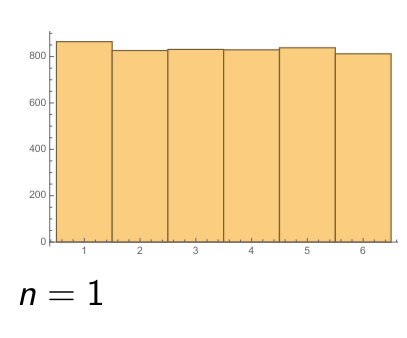
\includegraphics[width=\linewidth]{images/gauß_v10/n1}
        \end{subfigure}
        \hfill
        \begin{subfigure}[t]{0.24\textwidth}
            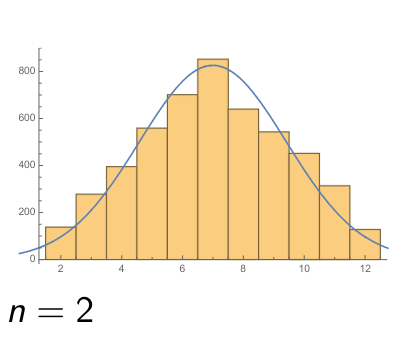
\includegraphics[width=\linewidth]{images/gauß_v10/n2}
        \end{subfigure}
        \hfill
        \begin{subfigure}[t]{0.24\textwidth}
            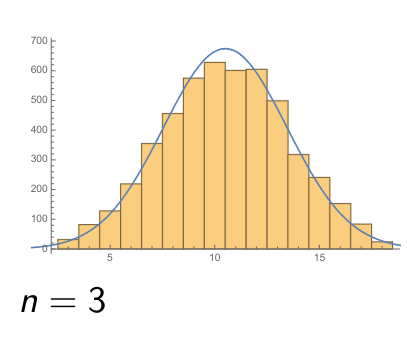
\includegraphics[width=\linewidth]{images/gauß_v10/n3}
        \end{subfigure}
        \hfill
        \begin{subfigure}[t]{0.24\textwidth}
            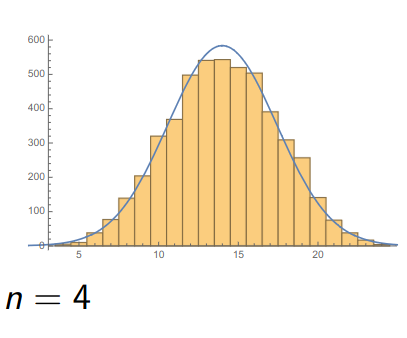
\includegraphics[width=\linewidth]{images/gauß_v10/n4}
        \end{subfigure}
        \hfill
        \begin{subfigure}[t]{0.24\textwidth}
            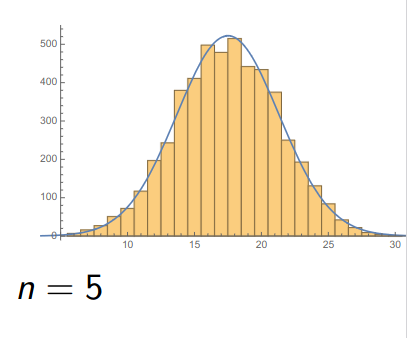
\includegraphics[width=\linewidth]{images/gauß_v10/n5}
        \end{subfigure}
        \hfill
        \begin{subfigure}[t]{0.24\textwidth}
            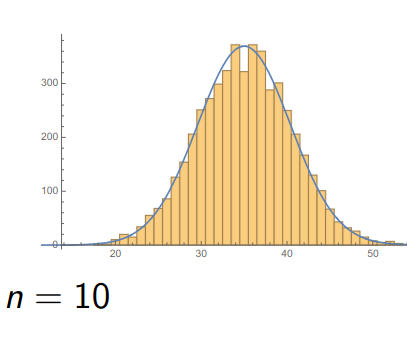
\includegraphics[width=\linewidth]{images/gauß_v10/n10}
        \end{subfigure}
        \hfill
        \begin{subfigure}[t]{0.24\textwidth}
            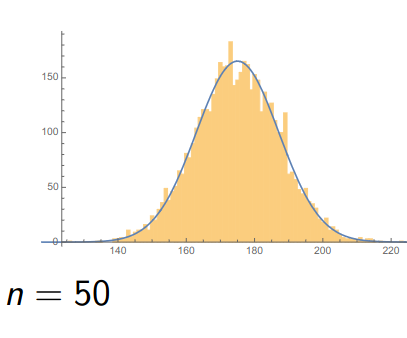
\includegraphics[width=\linewidth]{images/gauß_v10/n50}
        \end{subfigure}
        \hfill
        \begin{subfigure}[t]{0.24\textwidth}
            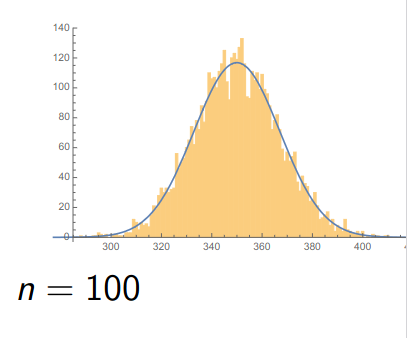
\includegraphics[width=\linewidth]{images/gauß_v10/n100}
        \end{subfigure}
    \end{figure}
\end{bsp}

\begin{satz}
    \textbf{Poissonscher Grenzwertsatz} \textit{Approximationen der Binomialverteilung} \txc{(2026)} \\
    Gilt $np_n \rightarrow \alpha > 0$ für $ n \rightarrow \infty$, so gilt für jedes feste $k \in \nz$
    \[
        \Binomv(k) \rightarrow \potm_{\alpha}(k) = \frac{\alpha^k}{k!} e^{- \alpha} \quad \text{ für } n \rightarrow \infty
    \]
    \paragraph{Beweis.} Sei k fest und  $np_n \rightarrow \alpha > 0$ für $ n \rightarrow \infty$. Daraus folgt
    insbesondere: $p_n \rightarrow 0$ für $ n \rightarrow \infty$.
    \begin{align*}
        \Binomv(k) & = \binom{n}{k} p_n^k (1-p_n)^{n-k} \\
        & = \frac{n(n - 1) . . . (n - k + 1)}{k!}  p_n^k (1-p_n)^{n-k} \\
        & = \oub{1 \cdot  (1  - \frac{1}{n}) \cdots  (1  - \frac{k-1}{n})}{\rightarrow 1} \oub{\frac{(np_n)^k}{k!}}{
            \rightarrow \frac{\alpha^k}{k!}} \oub{\left(  1 - \frac{np_n}{n} \right)^n }{\overset{*}{\rightarrow} e^{
            -\alpha}} \oub{\left( 1-p_n \right)^{-k}}{\rightarrow 1} \\
        & \rightarrow \frac{\alpha^k}{k!}  e^{-\alpha} \\
        & = \potm_{\alpha} (k)
    \end{align*}
    \txo{* $(1- \frac{\alpha_n}{n})^n \rightarrow e^{-\alpha}$ gilt auch für Folge $(\alpha_n)_n$(?) mit $\alpha_n \rightarrow \alpha$, nicht nur für feste $\alpha$.}
\end{satz}

\begin{bem}
    \textbf{Fehlerabschätzung / Güte der Approximation} \txc{(2026)} \\
    Gegeben $\sn$ binomialverteilt mit Parametern n und $p_n$ und $Z_{np_n}$ poisson-verteilt mit Parameter $np_n$.
    Angenommen $np_n \rightarrow \alpha$.
    Dann gilt die Abschätzung
    \[
        sup_{C \subset \nz_0} | \pe(\sn \in C) - \pe(Z_{np_n} \in C)| \leq 2np^2_n \txo{\ = 2 \underbrace{np_n}_{\rightarrow \alpha} p_n}
    \]
    Und für jede Konstante $K > 2$ und n groß genug gilt
    \[
        sup_{C \subset \nz_0} | \pe(\sn \in C) - \pe(Z_{np_n} \in C)| \leq K \alpha p_n \rightarrow 0 \quad \text{ für } n \rightarrow \infty
    \]
\end{bem}

\begin{bem}
    Die Poisson-Approximation ist gut, wenn n groß im Vergleich zu k ist ($n >> k$) und p klein ist (
    $n >> \alpha := np$).
    Das heißt insbesondere, daß die Erfolgswahrscheinlichkeit klein sein muss.
    % TODO für das untere auch karteikarte?
    Für derartige seltene Ereignisse verwenden wir $\pe (\sn = k) \approx \potm_{\alpha}(k)$ mit $\alpha := np$.
\end{bem}

\karkar{wann_poisson}

\begin{bsp}
    \textbf{Seltenes Ereignis / Roulette} \txc{(2026)} \\
    Wir betrachten ein Roulettespiel mit 36 ``Zahlen'' und einer ``Null''. \\
    Wir setzen immer auf eine bestimmte Zahl: p = 1/37 und wir tun dies n = 37 Mal.
    Das heißt, wir erwarten im Mittel einen Gewinn:$\alpha  = np = 1$. \\
    Wie groß ist die Ws., $ 0 \times, 1 \times, 2 \times, ...$ zu gewinnen?
    \begin{mytable}
        \begin{tabular}{ccc}
            k & $\Bnmv_{37,1/37}(k)$ & $\potm_1(k)$ \\
            0 & 0.363 & 0.368 \\
            1 & 0.363 & 0.368 \\
            2 & 0.186 &  0.184 \\
            $\vdots$ & $\vdots$ & $\vdots$ \\
            5&  0.00261 & 0.00306 \\
            $\vdots$ & $\vdots$ & $\vdots$ \\
            15  & $1.5 \cdot 10^{14} $ & $2.8 \cdot 10^{13}$
        \end{tabular} % todo wofür steht \potm_1(k)$ überhaupt und so?
    \end{mytable}
\end{bsp}

\begin{bsp}
    \textbf{Historisches Beispiel zur Poisson-Approximation: Tote durch Hufschlag in Preussen} \txc{(2026)} \\
    Vorliegende Daten: 10 Armeecorps über 20 Jahre,
    entspricht 200 Corps-Jahren.
    \begin{mytable}
        \begin{tabular}{|c|c|c|}
            \hline
            Tote $k$ & Anzahl Jahre mit $k$ Toten & $200 \cdot P_\varrho(k)$ mit $\varrho = 0{,}61$ \\
            \hline
            0 & 109 & 109 \\
            1 & 65  & 66  \\
            2 & 22  & 20  \\
            3 & 3   & 4   \\
            4 & 1   & 1   \\
            $\geq 5$ & 0 & 0 \\
            \hline
        \end{tabular}
        \caption{Die durch Schlag eines Pferdes im preussischen Heere Getöteten (Ladislaus von Bortkiewicz, Das Gesetz der kleinen Zahlen, Teubner (1898))}
    \end{mytable}
    Hier wurde $\alpha$ gewählt als die mittlere Anzahl an Toten pro (Corps-)Jahr:
    \[
        \alpha = (1 · 65 + 2 · 22 + 3 · 3 + 1 · 4)/200 = 0, 61
    \]
\end{bsp}

\begin{bsp}
    \textbf{Beispiel zur Poisson-Approximation: Zellzählung im Gitternetz} \txc{(2026)} \\
    Zellen unter dem Mikroskop, Gitternetz, im Schnitt $\nu$ Zellen pro kleinem Quadrat, N Quadrate.
    \paragraph{Modellierung:} Verteile $N \nu$ Zellen zufällig und unabhängig voneinander auf N Quadrate.
    Wahrscheinlichkeit $p = 1/N$ für eine Zelle, im vorab gewählten Quadrat $\varphi$ zu landen.
    Wahrscheinlichkeit k Zellen im Quadrat $\varphi$ zu finden, ist $\Bnmv_{N\nu , 1/N}(k)$. \\
    \[
        \txo{ np_n \equiv \nu
        \begin{cases}
            n  & = N \nu \\
            p_n & = \frac{1}{N}
        \end{cases}
        }
    \]
    Bei großer Zahl N von Quadraten gelten $N \nu >> k$ und $N \nu >> \oub{(N\nu)}{n}  \oub{\frac{1}{N}}{p_n} = \nu$. \\
    Poisson-Approximation zeigt $\Bnmv_{N\nu , 1/N}(k) \approx \potm_{\nu}(k)$. \\
    Dies rechtfertigt, eine derartige Verteilung von Zellen oder Teilchen mit Hilfe der
    Poisson-Verteilung zu modellieren.
\end{bsp}

\begin{bsp}
    \textbf{Beispiel zur Poisson-Approximation: Im zeitlichen Verlauf eintreffende Rechenaufträge} \txc{(2026)} \\
    Im Schnitt $\alpha$ eintreffende Rechenaufträge pro
    Zeiteinheit (z.B. pro Stunde) \\
    Ws., daß ein Auftrag eintrifft in einem sehr kleinen
    Zeitfenster der Länge $\delta << 1$ sei näherungsweise $\alpha \delta$.
    ($\delta$ sehr klein, z.B. eine Millisekunde)). \\
    Wir zerlegen das Gesamtzeitintervall $[0, t)$ in N sehr kleine, disjunkte
    Teilintervalle der Länge $t/N$. (für ein festes t, z.B. 30 Minuten, 24 Stunden, drei Wochen, . . . )
    \[
        [0, t) = \bigcup_{k=1}^N \left[  \frac{k-1}{N} \cdot t, \frac{k}{N} \cdot t \right)
    \]
    Ws., dass ein Auftrag eintrifft in einem bestimmten dieser Zeitfenster, ist
    näherungsweise $\alpha t / N$.
    \paragraph{Annahmen:} Für großes N sind die Zeitfenster so klein, daß wir annehmen dürfen, daß in
    jedem Fenster ein oder kein Auftrag eintrifft (d.h., wir schließen aus, daß mehr als ein Auftrag eintreffen kann)
    . Ob ein Auftrag in einem bestimmten Fenster eintrifft, sei unabhängig vom
    Eintreffen von Aufträgen in allen anderen Zeitfenstern.
    \paragraph{Modellierung:} Damit haben wir jedem Zeitfenster, d.h. jedem k, eine Bernoulli-Variable
    zugeordnet, die uns sagt, ob im zugehörigen Zeitfenster k ein Auftrag
    eintrifft.
    Die Erfolgsws. dieser Bernoulli-Variable ist $\alpha t / N$
    \txc{(Also die Ws, dass ein Auftrag in einem bestimmten Zeitfenster eintritt)}.
    Die Anzahl der Aufträge, die im Intervall $[0, t)$ eintreffen, ist binomialverteilt
    mit Parametern N und $\alpha t / N$.
    \[
        \txo{ n = N, \quad p_n = \frac{\alpha t}{N}  = \alpha t \frac{1}{N}}
    \]
    Für die Ws., insgesamt $\varphi$ Aufträge im Intervall $[0, t)$ zu haben, ergibt die
    Poisson-Approximation für große N:
    \[
        \Bnmv_{N, \alpha t / N}(\varphi) \approx \potm_{N \cdot \alpha t / N}(\varphi) = \potm_{\alpha t}(\varphi)
    \]
    (Beachten Sie, daß wir in diesem Problem N beliebig groß machen dürfen. Wir verwenden
    hier die beliebige Teilbarkeit der Zeit!) \\
    Wiederum rechtfertigt unsere Betrachtung, beim Modellieren derartiger Prozesse
    generell die Poisson-Verteilung zu verwenden.
\end{bsp}

% TODO geneinsamkeite und unterschiede Normal- und Poisson-Approximation / Diskussion

\begin{lem}
    \textbf{Poisson-Approximation für Erfolgswahrscheinlichkeit p nahe 1} \txc{(2026)} \\
    Betrachte die Anzahl Erfolge $\sn$ in einem unabhängig n-mal wiederholten
    Bernoulli-Experiment mit:
    \begin{itemize}
        \item n groß
        \item p nahe bei 1, d.h., q = 1 - p klein
    \end{itemize}
    Zusatzüberlegung erlaubt es, die Poisson-Approximation anzuwenden:
    Tausche die Rollen von ``Erfolg'' und ``Mißerfolg'' (zähle Mißerfolge !)\\
    $\tilde\sn = n - \sn$ zählt die Anzahl der ``Mißerfolge''  $\tilde\sn$ ist $\Bnmv_{n,q}$-verteilt. \\
    Sei $\tilde \alpha = \E{\tilde\sn} = nq$. \\
    Poisson-Approximation:
    \[
        \pe(\tilde\sn = k) = \Bnmv_{n,q}(k) \approx \potm_{\tilde\alpha}(k); \quad \forall k \in \nz_0
    \]
    ``Zurück übersetzen'': : Für alle $k \in \nz_0$ gilt:
    \[
        \pe(\sn = k) = \pe( \tilde\sn = n - k) = \Bnmv_{n,q}(n - k) \approx \potm_{\tilde\alpha}(n - k) = \frac{(nq)^{(n-k)}}{(n - k)!} e^{-nq}
    \]
    \txc{Also:}
    \[
        \txc{\pe(\sn = k) = \pe( (n - \sn) = n - k) = \Bnmv_{n,q}(n - k) \approx \potm_{\E{n - \sn}}(n - k) = \frac{(nq)^{(n-k)}}{(n - k)!} e^{-nq}}
    \]
    \txc{Bzw.:}
    \[
        \txc{\pe(\sn = k) = \pe( (n - \sn) = n - k) = \Bnmv_{n,q}(n - k) \approx \potm_{nq}(n - k) = \frac{(nq)^{(n-k)}}{(n - k)!} e^{-nq}}
    \]
\end{lem}
\subsection{Beispielaufgabe Laubfrosch} \txc{(2026)} \\
Ein Laubfrosch legt $n = 1000$ Eier.
Aus jedem Ei entwickelt sich mit der WS $p = \frac{1}{200}$ ein Frosch.
\begin{auf}
    \subsubsection*{Wahrscheinlichkeitsraum angeben und Modell rechtfertigen}
    \txo{Ziel: Wahrscheinlichkeit, dass sich höchstens zwei Frösche entwickeln.}
    \paragraph{Lösung:} $n = 1000$, $\eraum = \{0,1\}^{1000}$\\
    $\ele_i = 1$ bedeutet i-tes Ei entwickelt sich zum Frosch.
    \[
        \wfk(\ele) = p^{\sumEN \ele_i} (1-p)^{n- \sumEN \ele_i}  \faoio
    \]
    Annahme: Frösche entwickeln sich unabhängig voneinander mit gleicher Ws.
\end{auf}

\begin{auf}
    \subsubsection*{Zufallsvariable, die Anzahl der Frösche angbit, die Verteilung und ggf. Parameter}
    $\sn: \eraum \rightarrow \{ 0, ..., n \}$ und
    \[
        \sn(\ele) := \sumEN \ele_i \faoio
    \]
    Als Anzahl von Erfolgen in unabhängig wiederholten Bernoulli-Experimenten ist $\sn$ binomialverteilt mit
    Paramatern n und p.
\end{auf}


\begin{auf}
    \subsubsection*{Erwartungswert und Varianz}
    $\sn$ ist binomialverteilt mit Parametern n und p.
    Daher existieren EW und Varianz und es gilt:
    \[
        \E{\sn} = np  = 1000 \frac{1}{200} = 5
    \]
    und
    \[
        \Var(\sn) = np (1-p) = 5 \cdot (1 - \frac{1}{200}) = 5 \cdot \frac{199}{200} = \frac{199}{40}
    \]
\end{auf}


\begin{auf}
    \subsubsection*{WS. maximal zwei Frösche zu haben}
    \txo{$\alpha = pn = 5$}
    \begin{align*}
        \pe(\sn \leq 2 ) & = \pe(\sn = 0) + \pe(\sn = 1) + \pe(\sn = 2) \\
        & \approx \left[  \frac{\alpha^0}{0!} e^{-\alpha} +  \frac{\alpha^1}{1!} e^{-\alpha} +  \frac{\alpha^2}{2!}
                      e^{-\alpha}  \right] & Poiss.-Approx. \\
        & = \left[  1+5 + \frac{25}{2} \right] e^{-\alpha} & * \\
        & =  \left[  1+5 + \frac{25}{2} \right] e^{-5} & ** \\
    \end{align*}
    \begin{itemize}
        \item[*] n groß, $p = \frac{1}{200}$ klein
        \item[**] $k = 0,1,2$ klein gegenüber n
    \end{itemize}
\end{auf}

\begin{bem}
    \textbf{Bruchrechnung im Kontext der Binomialapproximation nicht ausmultiplizieren!} \txc{(2026)} \\
    Sondern mit Parametern rechnen und n und p so spät wie möglich einsetzen.
    % TODO EVTL Beispiel
\end{bem}



